\section{I. Voronoi-Diagramm}
\subsection{Grundlagen}
\begin{frame}{Voronoi-Diagramm}
 \begin{figure}[h]
 \centering
 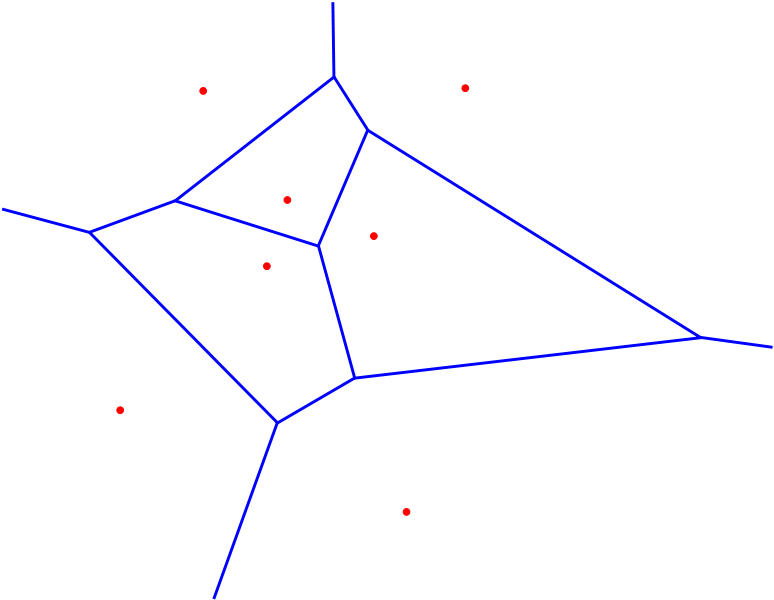
\includegraphics[width=0.4\textwidth]{./material/voronoi-step1-1.png}
 % complete.png: 845x703 pixel, 72dpi, 29.81x24.80 cm, bb=0 0 845 703
 \caption{Voronoi-Diagramm Wikipedia}
%  \label{fig:gesamt}
\end{figure}
\begin{description}
 \item[Voronoi-Diagramm] Linien in eine Punktwolke legen, so dass die Linien zu 2 Punkten immer denselben Abstand haben
 \item[Verallgemeinertes Voronoi-Diagramm] Statt der Punktwolke können auch Linien verwendet werden
\end{description}

\end{frame}

\subsection{Algorithmus}
\begin{frame}{Voronoi-Diagramm - 1. Berechnung des GVG}
  nach \cite{Thrun1998}

\begin{figure}[h]
 \centering
 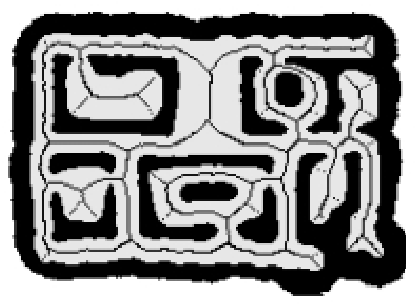
\includegraphics[width=0.6\textwidth]{./material/voronoi-step1.png}
 % complete.png: 845x703 pixel, 72dpi, 29.81x24.80 cm, bb=0 0 845 703
 \caption{Voronoi Schritt 1 \cite{Thrun1998}}
%  \label{fig:gesamt}
\end{figure}

% Voronoi Diagramm: 
% Verallgemeinertes Voronoi-Diagramm: Statt einfache Punkte können auch Linien verwendet werden
\end{frame}
\begin{frame}{Voronoi-Diagramm - 2. Kritische Linien}
\begin{figure}[h]
 \centering
 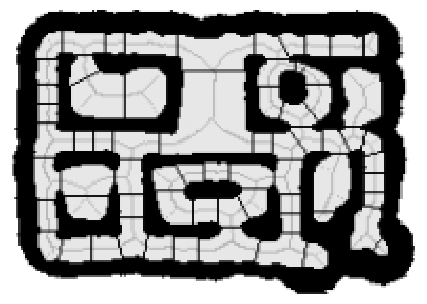
\includegraphics[width=0.6\textwidth]{./material/voronoi-step2.png}
 % complete.png: 845x703 pixel, 72dpi, 29.81x24.80 cm, bb=0 0 845 703
 \caption{Voronoi Schritt 2: Kritische Punkte/Linien \cite{Thrun1998}}
%  \label{fig:gesamt}
\end{figure}
Diejenigen Punkte auf dem Diagramm, die lokal einen geringen Abstand zur Wand besitzen
  
\end{frame}
\begin{frame}{Voronoi-Diagramm - Weitere Schritte}
 \begin{figure}[h]
 \centering
 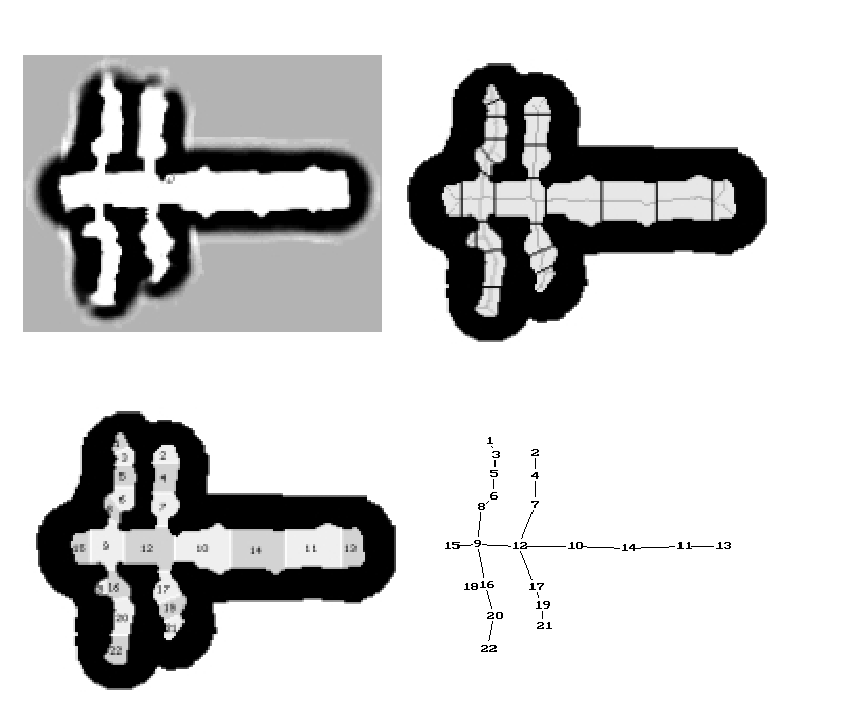
\includegraphics[width=0.65\textwidth]{./material/complete.png}
 % complete.png: 845x703 pixel, 72dpi, 29.81x24.80 cm, bb=0 0 845 703
 \caption{Übersicht \cite{Thrun1998}}
 \label{fig:gesamt}
\end{figure}
 
\end{frame}
\subsection{Probleme}
\begin{frame}{Probleme}
 \begin{itemize}
  \item Nachbarschaftssuche ist sehr aufwändig $\to$ sehr viele Papers mit Optimierungen
  \item Schwache Kreuzungen und Boundary Edges
 \end{itemize}
\begin{figure}[h]
 \centering
 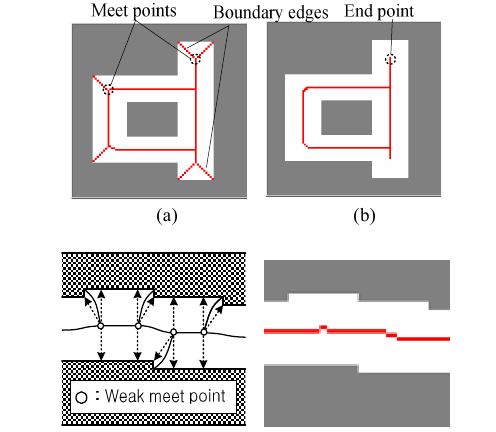
\includegraphics[width=0.5\textwidth]{./material/thinningvsvoronoi.png}
 % thinningvsvoronoi.png: 496x485 pixel, 72dpi, 17.50x17.11 cm, bb=0 0 496 485
 \caption{Voronoi vs. Thinning \cite{KoBangYun}}
 \label{fig:egal}
\end{figure}

 
\end{frame}
